\section{Hlavní stránka}

\label{nur:homepage}
Stránka obsahuje rozvržení webu s mapou. Podoba stránky jde vidět na obrázku \ref{fig:tur:homepage}

\begin{figure}[h]
    \centering
    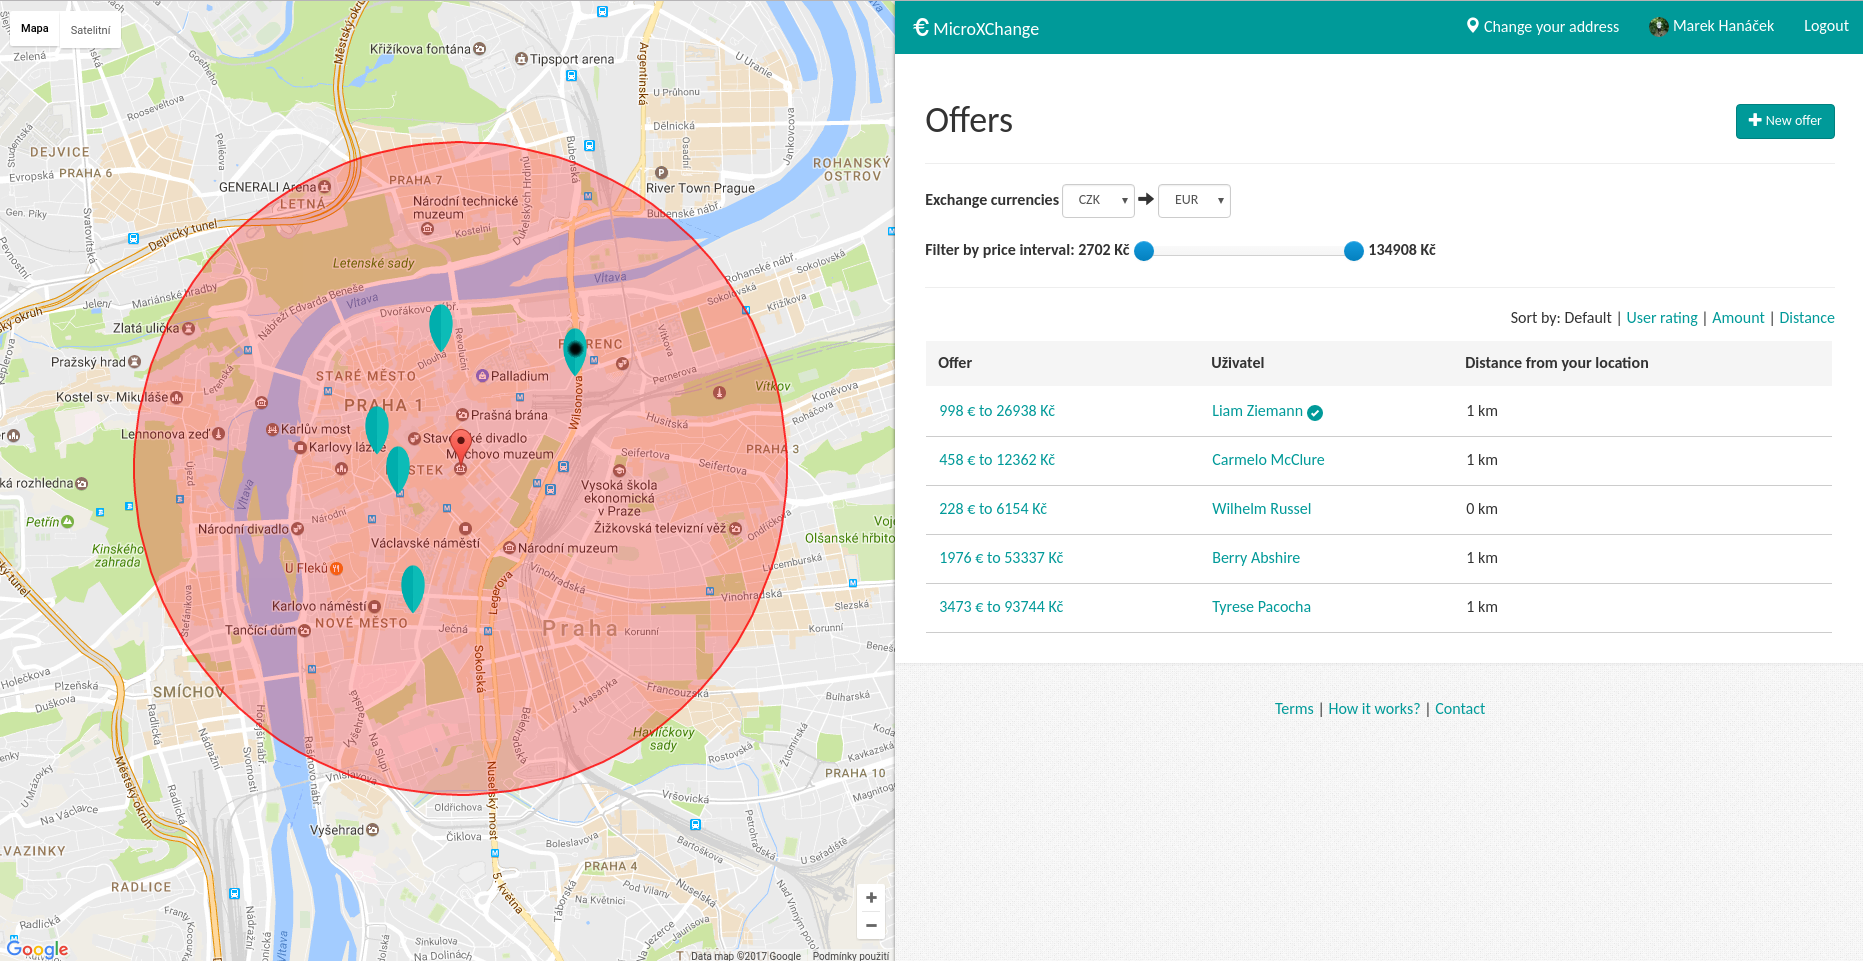
\includegraphics[width=1.0\textwidth]{media/tur/homepage.png}
    \caption{Hlavní stránka aplikace}
    \label{fig:tur:homepage}
\end{figure}

\subsection{Mapa}
Mapa obsahuje ukazatel polohy uživatele, kruh znázorňující vyhledávací rádius a ukazatele poloh nabídek. Ukazatele poloh nabídek jsou dvojího typu: nabídky od ověřených uživatelů a nabídky od ostatních uživatelů.
\\\\
Nabídky jsou také zobrazeny v textové části, jelikož v mapě se špatně filtruje a řadí nabídky.

\subsection{Textová část}
Textová část se skládá z hlavičky, filtračního formuláře, seznamu nabídek s možností seřazení, tlačítka pro vytvoření nové nabídky a patičky obsahující odkazy na informační stránky.

\subsection{Filtrace nabídek}
Formulář obsahuje tři základní parametry pomocí nichž lze filtrovat:
\begin{itemize}
	\item Měnu ze které chceme peníze směnit,
	\item měnu do které chceme peníze směnit a
	\item interval obnosu peněz.
\end{itemize}
Filtrace dále bere v potaz i aktuální, respektive uživatelem zadanou polohu, a rádius. Filtrace se samozřejmě projevuje i v mapě. Jsou tedy zobrazeny jen ty nabídky, které odpovídají zadaným filtrům.

\subsection{Řazení nabídek}
Vidno na obrázku \ref{fig:tur:sorting}. Nabídky lze seřadit čtyřmi různými způsoby:
\begin{itemize}
	\item Vzestupně dle vzdálenosti uživatelovy polohy od centra nabídky.
	\item Vzestupně dle obnosu peněz nabídek.
	\item Sestupně dle hodnocení uživatelů.
	\item Dle kombinace více kritérií nabídek. Tento způsob blíže popisuji v následující sekci.
\end{itemize}

\begin{figure}[h]
    \centering
    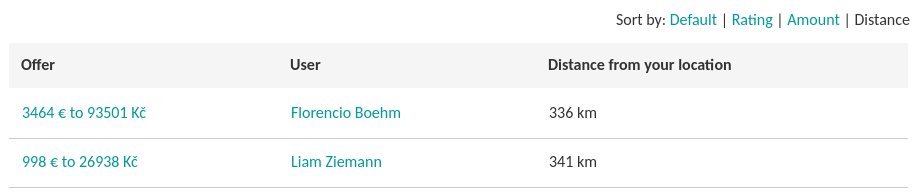
\includegraphics[width=1.0\textwidth]{media/tur/sorting.png}
    \caption{Výpis nabídek s možností seřazení}
    \label{fig:tur:sorting}
\end{figure}

\subsubsection{Řazení dle kombinace více kritérií nabídek}
Hodnocení se skládá ze 2 složek:
\begin{itemize}
	\item Hodnocení uživatele
        \begin{itemize}
            \item Jestliže uživatel má měně jak 2 hodnocení, pak je tato hodnota rovna 0
            \item Jestliže uživatel má více než 2 hodnocení, pak se hodnota odvíjí od průměrného počtu hvězdiček. Konkrétně:
            \begin{itemize}
                \item 0 hvězdiček $\rightarrow$ penalizace -2
                \item 1 hvězdiček $\rightarrow$ penalizace -1.5
                \item 2 hvězdiček $\rightarrow$ penalizace -1
                \item 3 hvězdiček $\rightarrow$ hodnocení je rovno 0.6
                \item 4 hvězdiček $\rightarrow$ hodnocení je rovno 0.8
                \item 5 hvězdiček $\rightarrow$ hodnocení je rovno 1
            \end{itemize}
        \end{itemize}
	\item Vzdálenost od uživatele
        \begin{itemize}
            \item Za vzdálenost od uživatele může nabídka dostat 0 až 1 bod.
            \item Hodnota se počítá na základě minimální a maximální vzdálenosti nabídek od něj. Tento interval normalizuji na interval od 0 do 1 a stejně tak pak vzdálenost nabídky od uživatele. Konkrétně to lze vidět na ukázce kódu \ref{code:sorting-distance}
            \item Pokud budu mít například 3 nabídky ve vzdálenostech 15~km, 2~km a 28~km, tak hodnocení budou 0.5, 1 a 0.
        \end{itemize}
\end{itemize}

\begin{listing}[htbp]
\caption{\label{code:sorting-distance}Funkce výpočet hodnocení vzdálenosti od uživatele}
\begin{minted}[frame=lines,bgcolor=codebg,fontsize=\footnotesize,linenos,breaklines]{Python}
def get_distance_rating(offer, min_distance, min_max_distance):
    distance_from_min = offer.distance_from_user - min_distance
    percent = min_max_distance / 100
    return 1 - ((distance_from_min / percent) / 100)
\end{minted}
\end{listing}

\subsection{Mobilní verze}
Stejně jako při návrhu desktopové verze tak i při návrhu mobilní verze se inspiruji webem SReality.cz, který jsem analyzoval v sekci \ref{analyza:sreality}. Zobrazuje se tedy vždy pouze mapa nebo textová část. Viz. obrázek \ref{fig:tur:homepage-mobile}.

\begin{figure}[h]
    \centering
    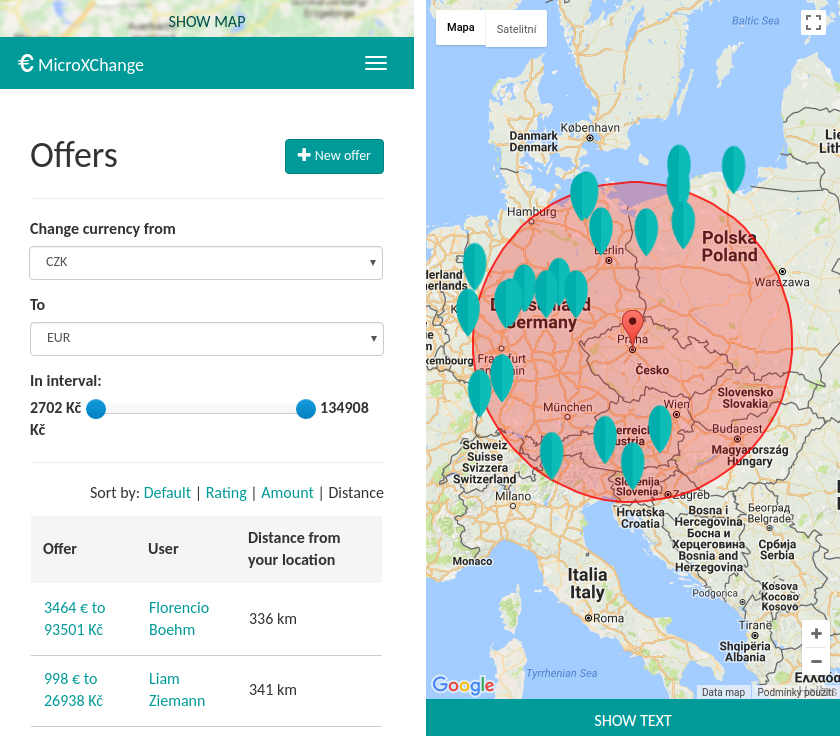
\includegraphics[width=1.0\textwidth]{media/tur/homepage-mobile.png}
    \caption{Mobilní verze aplikace}
    \label{fig:tur:homepage-mobile}
\end{figure}
